\section{Introduction}
\label{introduction}

Recent years, social media platforms have seen a rapid growth of user-generated multimedia contents. Billion of images are shared on multiple social media platforms such as Instagram or Twitter which contributes to a large portion of the shared links. Through image sharing, users are usually also express their emotions and sentiments to strengthen the opinion carried in the content. Understanding users' sentiments provide us reliable signals of people's real-world activities which are very helpful in many applications such as predicting movie box-office revenues \cite{asur2010predicting}, political voting forecasts \cite{o2010tweets}. It can also be used as the building block for other tasks such as the image captioning \cite{vinyals2015show}.

Automatic sentiment analysis recognizes a person's position, attitude or opinion on an entity with computer technologies \cite{soleymani2017survey}. Text-based sentiment analysis has been the main concentration in the past. Only recently, sentiment analysis from online social media images has begun to draw more attentions. To simplify the task, previously, the sentiment analysis mainly focuses on the opinion's polarity, i.e., one's sentiment is classified into categories of positive, neutral and negative. 
However, as pointed out in many recent studies \cite{borth2013large, yuan2013sentribute, chen2014deepsentibank, ahsan2017towards}, it faces the unique challenge of large "affective gap" between the low-level features and the high-level sentiments. 

\begin{figure}[h]
    \centering
    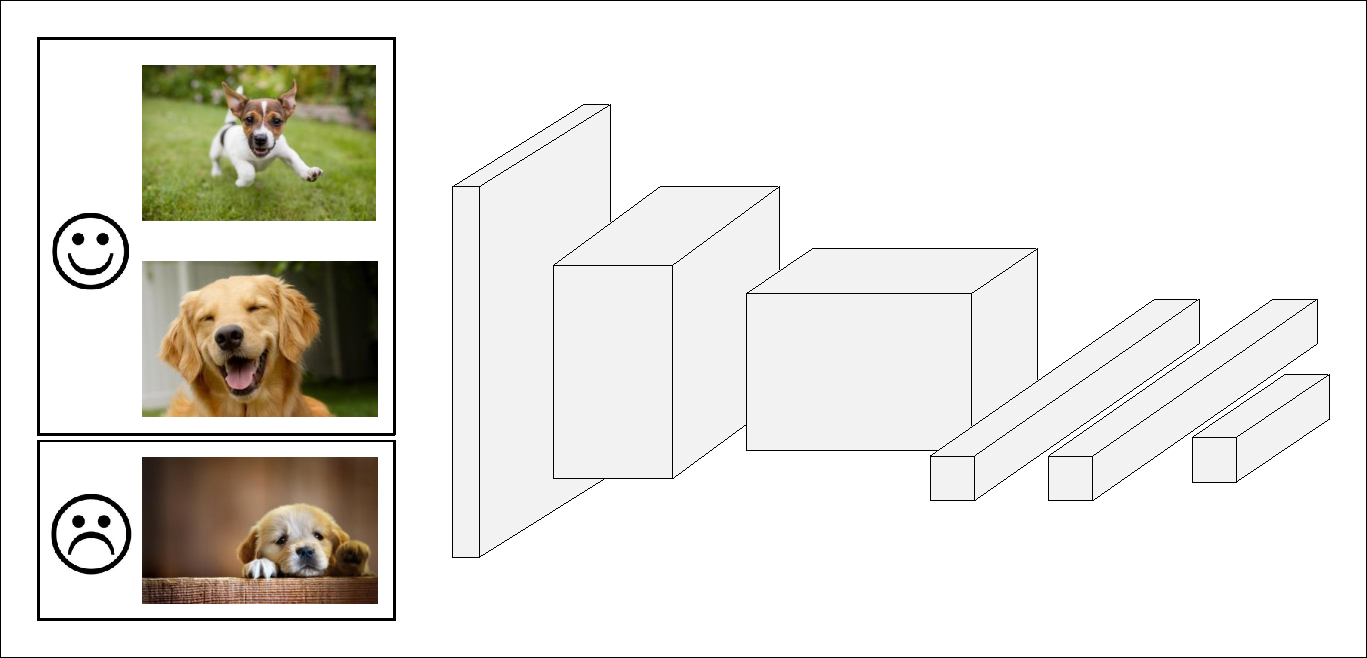
\includegraphics[width=\linewidth]{./figures/intro.pdf}
    \caption{Image sentiment analysis with triplet loss}
    \label{fig:intro}
\end{figure}

Recent work resort to extract manually designed mid-level representations from low-level features for image sentiment analysis tasks, e.g., visual sentiment ontology (VSO) in \cite{borth2013large}, mid-level attributes in \cite{yuan2013sentribute}. Such mid-level representations usually include both adjective and noun parts such as "happy dogs", "creepy house" and have strong sentiment. So approaches based on mid-level representations usually outperforms methods that inferring sentiment directly from low-level features. Rapid developments in Convolutional Neural Network (CNN) \cite{krizhevsky2012imagenet, szegedy2015going, simonyan2014very, he2016deep} push the transformations of computer vision tasks. There are also several efforts to apply CNN to image sentiment analysis \cite{you2015robust, chen2014deepsentibank, campos2017pixels}. However, recent works on applying convolutional networks still borrow the network architectures from the image classification tasks \cite{you2015robust, chen2014deepsentibank, ahsan2017towards, campos2017pixels}. Although convolutional neural networks are very effective at image classification tasks, they are not as effective when separating adjective parts that widely found in most mid-level representations for image sentiment analysis purpose.

To overcome this challenge, we first let the convolutional neural network trained on the noun part, then we adopt the triplet loss to replace surrogate loss used in the convolutional neural networks to force the network to focus more on the adjective part in the mid-level representations. When applying triplet loss, the network loot at three data points at the same time, the anchor point, the positive point and the negative point, where the anchor point and the positive point belongs to the same class and the negative point belongs to a different class. Then during training, the network tries to minimize the distance between anchor point and positive point and maximize the distance between the anchor point and the negative point.

A major challenge for triplet loss is mining triplets, as trivial triplets are not uninformative to the network and too hard triplets make the network hard to learn "normal" features \cite{hermans2017defense}. When applying triplet loss to mid-level representation classification for image sentiment analysis, we select triplets from the same noun class, with the anchor point and the positive point belongs to the same adjective class while negative point belongs to a different adjective class. In this way, the triplet loss forces the network to learn the adjective part of the mid-level representations and the triplets are informative and moderately hard for the network to learn.
  
\subsection{Contributions}
Our contributions can be summarized as follows:

\begin{itemize}
	\item We apply a two-stage learning scheme for the network to learn the adjective and noun part of mid-level representations in the image sentiment analysis separately;
	\item We replace surrogate loss in convolutional neural networks with triplet loss and design a triplet selection approach to force the network learn the adjective part of mid-level representations;
	\item We perform extensive experiments on several real word datasets to show the effectiveness of our approach in both mid-level representation classification and sentiment prediction.
\end{itemize}

The rest of this paper is organized as follows. In Section~\ref{relatedwork} we show previous works on image sentiment analysis.  
We explain our system structure and triplet selection scheme in Section~\ref{design}. 
The evaluations of our proposed method are in Section~\ref{evaluation}. 
We conclude our work in Section~\ref{conclusion}.
